\section{Data Acquisition}
\label{sec:chap_slam_data_acquisition}

In the following section, we first describe the robotic platform and sensors used to gather our place recognition dataset. We then describe in more details the dataset acquisition procedure and the resulting data.


\subsection{Robotic platform}
\label{ssec:chap_slam_platform}

The Husky A200 is a medium size (990 x 670 x 390 \SI{28}{\milli\meter}) \gls{ugv} developed by Clearpath Robotics~\cite{ClearpathWeb}. It is a rugged robot designed for all terrain conditions, therefore well suited for our experiments in forest. It uses a differential-drive skid steer allowing easy control and in place turns for our data acquisition. It has a maximum speed of \SI{1}{\meter\per\second}, but we generally acquire data at lower speed, which minimizes odometry and range data error. This platform, with a maximum payload capability of \SI{75}{\kilo\gram}, can easily carry all sensors used for our experiments. Table~\ref{tab:husky_sensors} show a complete list of sensors available on the platform.

For our place recognition research, we mainly use the wheel encoder along with the \gls{imu} for odometry
\begin{itemize}
    \item Talk about the onboard computer (run nodes, record data) communication via ssh.
    \item
\end{itemize}

\begin{figure}
    \centering
    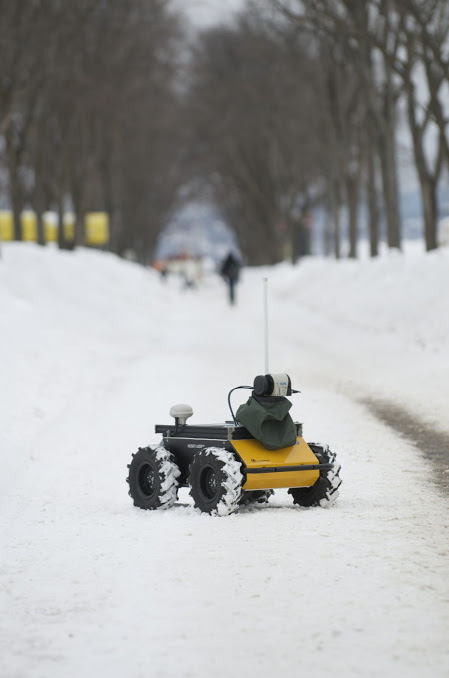
\includegraphics[width=0.95\linewidth]{img/chap_slam/husky.jpg}
    \caption{Wow such robot. \emph{Photo credit:} François Pomerleau}
    \label{fig:chap_slam_husky}
\end{figure}

\begin{table}[h]
    \centering
    \begin{tabular}{|c|c|c|c|}
        \hline
        \textbf{Sensor} & \textbf{Manufacturer/Model}       & \textbf{Data type}           & \textbf{Precision and/or} \\
                        &                                   &                              & \textbf{resolution}       \\ \hline
        Camera          & Axis / M1013                      & Photo                        & 640x480 pixels            \\ \hline
        \gls{lidar}     & SICK / LMS151                     & Nuage de point               & $\pm$ 0,04 mètre          \\
                        & Velodyne / HDL-32E                & tridimensionnel              & 0,25 degré                \\ \hline
        \gls{imu}       & ChRobotics / UM6                  & Accélérations et             & Inconnue                  \\
                        &                                   & vitesses angulaires          & Inconnue                  \\ \hline
        Motor current   & remove ?                          & Mesure du couple moteur      & Inconnue                  \\ \hline
        Wheel encoder   &                                   & Position angulaire des roues & 200000 impulsions         \\
                        &                                   &                              &  par mètre                \\ \hline
        \gls{gps}       & NovAtel / SMART6                  & Coordonnées                  & 0,18 mètre                \\
                        &                                   & géographiques                &                           \\ \hline
    \end{tabular}
    \caption{\label{tab:husky_sensors} \todo{Maybe broader\dots like payloads or devices. Add ptu, embedded computer}Set of sensors available on the Husky A200. Note that both \gls{lidar}s are not mounted at the same time,}
    \label{tab:husky_sensors}
\end{table}

\subsection{Dataset}
\begin{figure}[htpb]
    \centering
    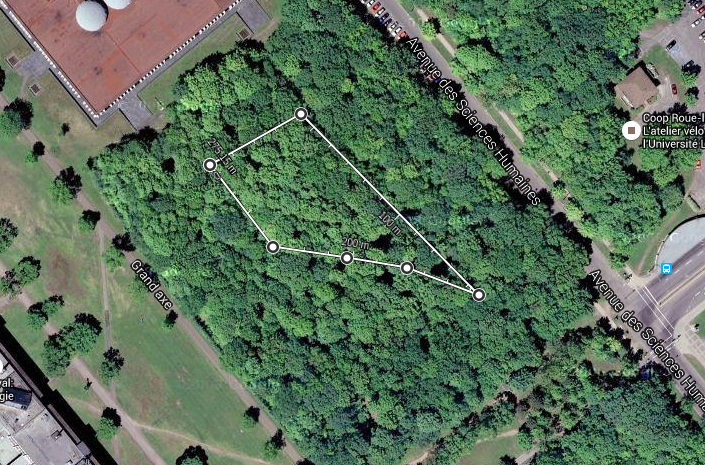
\includegraphics[width=0.95\linewidth]{img/chap_slam/path.png}
    \caption{Aerial view of the approximate path followed by the robot for data acquisition. Source: Google Maps, (2015)}
    \label{fig:chap_slam_path}
\end{figure}


\subsection{Dataset description}
\label{ssec:chap_slam_platform}

\begin{itemize}
    \item Communication to onboard computer via ssh.
    \item There run nodes and record data (data synchronization).
    \item All data is post-processed (semi important)
    \item SICK LMS151 vs velodyne (angles/density)
    \item Building(\todo{Should do the google map also}) vs forest
\end{itemize}
